\documentclass[twoside]{book}

% Packages required by doxygen
\usepackage{fixltx2e}
\usepackage{calc}
\usepackage{doxygen}
\usepackage[export]{adjustbox} % also loads graphicx
\usepackage{graphicx}
\usepackage[utf8]{inputenc}
\usepackage{makeidx}
\usepackage{multicol}
\usepackage{multirow}
\PassOptionsToPackage{warn}{textcomp}
\usepackage{textcomp}
\usepackage[nointegrals]{wasysym}
\usepackage[table]{xcolor}

% Font selection
\usepackage[T1]{fontenc}
\usepackage[scaled=.90]{helvet}
\usepackage{courier}
\usepackage{amssymb}
\usepackage{sectsty}
\renewcommand{\familydefault}{\sfdefault}
\allsectionsfont{%
  \fontseries{bc}\selectfont%
  \color{darkgray}%
}
\renewcommand{\DoxyLabelFont}{%
  \fontseries{bc}\selectfont%
  \color{darkgray}%
}
\newcommand{\+}{\discretionary{\mbox{\scriptsize$\hookleftarrow$}}{}{}}

% Page & text layout
\usepackage{geometry}
\geometry{%
  a4paper,%
  top=2.5cm,%
  bottom=2.5cm,%
  left=2.5cm,%
  right=2.5cm%
}
\tolerance=750
\hfuzz=15pt
\hbadness=750
\setlength{\emergencystretch}{15pt}
\setlength{\parindent}{0cm}
\setlength{\parskip}{3ex plus 2ex minus 2ex}
\makeatletter
\renewcommand{\paragraph}{%
  \@startsection{paragraph}{4}{0ex}{-1.0ex}{1.0ex}{%
    \normalfont\normalsize\bfseries\SS@parafont%
  }%
}
\renewcommand{\subparagraph}{%
  \@startsection{subparagraph}{5}{0ex}{-1.0ex}{1.0ex}{%
    \normalfont\normalsize\bfseries\SS@subparafont%
  }%
}
\makeatother

% Headers & footers
\usepackage{fancyhdr}
\pagestyle{fancyplain}
\fancyhead[LE]{\fancyplain{}{\bfseries\thepage}}
\fancyhead[CE]{\fancyplain{}{}}
\fancyhead[RE]{\fancyplain{}{\bfseries\leftmark}}
\fancyhead[LO]{\fancyplain{}{\bfseries\rightmark}}
\fancyhead[CO]{\fancyplain{}{}}
\fancyhead[RO]{\fancyplain{}{\bfseries\thepage}}
\fancyfoot[LE]{\fancyplain{}{}}
\fancyfoot[CE]{\fancyplain{}{}}
\fancyfoot[RE]{\fancyplain{}{\bfseries\scriptsize Generated by Doxygen }}
\fancyfoot[LO]{\fancyplain{}{\bfseries\scriptsize Generated by Doxygen }}
\fancyfoot[CO]{\fancyplain{}{}}
\fancyfoot[RO]{\fancyplain{}{}}
\renewcommand{\footrulewidth}{0.4pt}
\renewcommand{\chaptermark}[1]{%
  \markboth{#1}{}%
}
\renewcommand{\sectionmark}[1]{%
  \markright{\thesection\ #1}%
}

% Indices & bibliography
\usepackage{natbib}
\usepackage[titles]{tocloft}
\setcounter{tocdepth}{3}
\setcounter{secnumdepth}{5}
\makeindex

% Hyperlinks (required, but should be loaded last)
\usepackage{ifpdf}
\ifpdf
  \usepackage[pdftex,pagebackref=true]{hyperref}
\else
  \usepackage[ps2pdf,pagebackref=true]{hyperref}
\fi
\hypersetup{%
  colorlinks=true,%
  linkcolor=blue,%
  citecolor=blue,%
  unicode%
}

% Custom commands
\newcommand{\clearemptydoublepage}{%
  \newpage{\pagestyle{empty}\cleardoublepage}%
}

\usepackage{caption}
\captionsetup{labelsep=space,justification=centering,font={bf},singlelinecheck=off,skip=4pt,position=top}

%===== C O N T E N T S =====

\begin{document}

% Titlepage & ToC
\hypersetup{pageanchor=false,
             bookmarksnumbered=true,
             pdfencoding=unicode
            }
\pagenumbering{roman}
\begin{titlepage}
\vspace*{7cm}
\begin{center}%
{\Large My Project }\\
\vspace*{1cm}
{\large Generated by Doxygen 1.8.11}\\
\end{center}
\end{titlepage}
\clearemptydoublepage
\tableofcontents
\clearemptydoublepage
\pagenumbering{arabic}
\hypersetup{pageanchor=true}

%--- Begin generated contents ---
\chapter{File Index}
\section{File List}
Here is a list of all files with brief descriptions\+:\begin{DoxyCompactList}
\item\contentsline{section}{\hyperlink{Lab1_8c}{Lab1.\+c} }{\pageref{Lab1_8c}}{}
\end{DoxyCompactList}

\chapter{File Documentation}
\hypertarget{FinalLab_8cpp}{}\section{Final\+Lab.\+cpp File Reference}
\label{FinalLab_8cpp}\index{Final\+Lab.\+cpp@{Final\+Lab.\+cpp}}
{\ttfamily \#include $<$stdio.\+h$>$}\\*
{\ttfamily \#include $<$iostream$>$}\\*
{\ttfamily \#include $<$fstream$>$}\\*
{\ttfamily \#include $<$stdlib.\+h$>$}\\*
{\ttfamily \#include $<$string$>$}\\*
{\ttfamily \#include $<$vector$>$}\\*
{\ttfamily \#include $<$cmath$>$}\\*
{\ttfamily \#include $<$sstream$>$}\\*
Include dependency graph for Final\+Lab.\+cpp\+:
\nopagebreak
\begin{figure}[H]
\begin{center}
\leavevmode
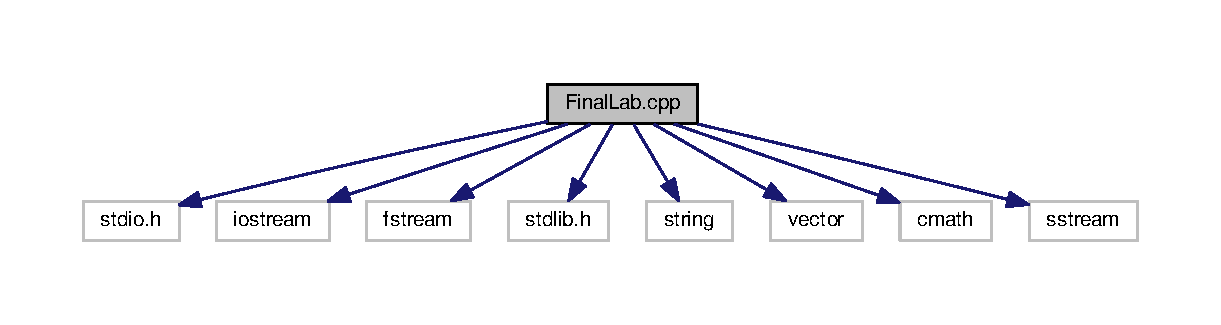
\includegraphics[width=350pt]{FinalLab_8cpp__incl}
\end{center}
\end{figure}
\subsection*{Functions}
\begin{DoxyCompactItemize}
\item 
int \hyperlink{FinalLab_8cpp_a0ddf1224851353fc92bfbff6f499fa97}{main} (int argc, char $\ast$argv\mbox{[}$\,$\mbox{]})
\end{DoxyCompactItemize}
\subsection*{Variables}
\begin{DoxyCompactItemize}
\item 
int \hyperlink{FinalLab_8cpp_a395b0fb68a5628e06819cb4aa43631fe}{M\+A\+X\+\_\+\+S\+I\+ZE} = 32
\end{DoxyCompactItemize}


\subsection{Function Documentation}
\index{Final\+Lab.\+cpp@{Final\+Lab.\+cpp}!main@{main}}
\index{main@{main}!Final\+Lab.\+cpp@{Final\+Lab.\+cpp}}
\subsubsection[{\texorpdfstring{main(int argc, char $\ast$argv[])}{main(int argc, char *argv[])}}]{\setlength{\rightskip}{0pt plus 5cm}int main (
\begin{DoxyParamCaption}
\item[{int}]{argc, }
\item[{char $\ast$}]{argv\mbox{[}$\,$\mbox{]}}
\end{DoxyParamCaption}
)}\hypertarget{FinalLab_8cpp_a0ddf1224851353fc92bfbff6f499fa97}{}\label{FinalLab_8cpp_a0ddf1224851353fc92bfbff6f499fa97}

\begin{DoxyCode}
26 \{
27    \textcolor{comment}{// must have exactly 2 arguments (a.out and the path to the directory)                                  
                                                                                                       }
28    \textcolor{keywordflow}{if}(argc =! 2)
29    \{
30       cerr << \textcolor{stringliteral}{"Error! Incorect number of arguments\(\backslash\)n"};
31       \textcolor{keywordflow}{return} -1;
32    \}
33 
34    \textcolor{comment}{// system call to get all files in argv[1] directory                                                    
                                                                                                       }
35    \textcolor{keywordtype}{string} s = argv[1];
36    system((\textcolor{stringliteral}{"ls -Rl "} + s + \textcolor{stringliteral}{" | grep ^- > output.txt"}).c\_str());
37 
38    \textcolor{comment}{//just get the file size and put it in a vector                                                         
                                                                                                       }
39    \textcolor{keywordtype}{string} line = \textcolor{stringliteral}{""};
40    \textcolor{keywordtype}{int} i = 1, k = 0;
41    vector<int> v;
42    ifstream in(\textcolor{stringliteral}{"output.txt"});
43    \textcolor{keywordflow}{while}(in >> line)
44    \{
45       \textcolor{keywordflow}{if}(i==5)
46       \{
47          k = atoi(line.c\_str());
48          v.push\_back(k);
49       \}
50       i++;
51       \textcolor{keywordflow}{if}(i>9)
52          i=1;
53    \}
54 
55    \textcolor{comment}{//count the number of files of a certain size and document in an array                                  
                                                                                                       }
56    \textcolor{comment}{//ex: if the size is 50, place in the 7th spot in array (32-64)                                         
                                                                                                       }
57    \textcolor{keywordtype}{int} num[\hyperlink{FinalLab_8cpp_a395b0fb68a5628e06819cb4aa43631fe}{MAX\_SIZE}] = \{0\};
58    \textcolor{keywordtype}{int} result;
59    \textcolor{keywordflow}{for}(\textcolor{keywordtype}{int} j = 0; j < v.size(); j++)
60    \{
61       \textcolor{keywordtype}{double} temp = v[j];
62       \textcolor{keywordflow}{if}(v[j] == 0)
63       \{
64          result = 0;
65          num[result] = num[result] + 1;
66       \} \textcolor{keywordflow}{else} \{
67          result = ilogb(temp); \textcolor{comment}{// finds closest 2^power                                                    
                                                                                                       }
68          num[result+1] = num[result+1] + 1;
69       \}
70    \}
71 
72    \textcolor{comment}{//writes the range, nuber of files, and percentage to a file                                            
                                                                                                       }
73    ofstream out;
74    \textcolor{keywordtype}{string} str = \textcolor{stringliteral}{""};
75    out.open(\textcolor{stringliteral}{"excel.txt"});
76    \textcolor{keywordflow}{if}(out.is\_open())
77    \{
78       out << \textcolor{stringliteral}{"range(KB):num\_of\_files:percentage(%)\(\backslash\)n"};
79       \textcolor{keywordflow}{for}(\textcolor{keywordtype}{int} j=0; j<\hyperlink{FinalLab_8cpp_a395b0fb68a5628e06819cb4aa43631fe}{MAX\_SIZE}; j++)
80       \{
81          \textcolor{keywordtype}{string} n=\textcolor{stringliteral}{""}, p=\textcolor{stringliteral}{""}, c=\textcolor{stringliteral}{""}, f=\textcolor{stringliteral}{""};
82          \textcolor{keywordflow}{if}(j==0) \textcolor{comment}{//if the file size is 0                                                                  
                                                                                                       }
83          \{
84             n = to\_string(num[j]);
85             p = to\_string((\textcolor{keywordtype}{double})num[j]/v.size()*100);
86             str = \textcolor{stringliteral}{"0-1:"} + n + \textcolor{stringliteral}{":"} + p + \textcolor{stringliteral}{"\(\backslash\)n"};
87          \} \textcolor{keywordflow}{else} \{ \textcolor{comment}{//if file size is greater than 0                                                         
                                                                                                       }
88             n = to\_string(num[j]); \textcolor{comment}{//number of files of certain size                                       
                                                                                                       }
89             p = to\_string((\textcolor{keywordtype}{double})num[j]/v.size()*100); \textcolor{comment}{// percentage}
90             \textcolor{comment}{//this is for the range                                                                        
                                                                                                       }
91             f = to\_string(((\textcolor{keywordtype}{int})pow(2.0, j)));
92             c = to\_string(((\textcolor{keywordtype}{int})pow(2.0, (j-1))));
93             \textcolor{keywordflow}{if}(j == 31)
94                str = str + c + \textcolor{stringliteral}{""} + f + \textcolor{stringliteral}{":"} + n + \textcolor{stringliteral}{":"} + p + \textcolor{stringliteral}{"\(\backslash\)n"};
95             \textcolor{keywordflow}{else}
96                str = str + c + \textcolor{stringliteral}{"-"} + f + \textcolor{stringliteral}{":"} + n + \textcolor{stringliteral}{":"} + p + \textcolor{stringliteral}{"\(\backslash\)n"};
97          \}
98       \}
99       out << str; \textcolor{comment}{//writes string str to file                                                              
                                                                                                       }
100       out.close();
101    \}
102    \textcolor{keywordflow}{else}
103    \{
104       cerr << \textcolor{stringliteral}{"Could not open file\(\backslash\)n"};
105       \textcolor{keywordflow}{return} -1;
106    \}
107 
108    \textcolor{comment}{// display the file on the terminal                                                                     
                                                                                                       }
109    system(\textcolor{stringliteral}{"awk -F\(\backslash\)":\(\backslash\)" '\{printf \(\backslash\)"%-25s %-20s %-20s\(\backslash\)\(\backslash\)n\(\backslash\)", $1,$2,$3\}' excel.txt"});
110 
111    \textcolor{keywordflow}{return} 0;
112 \}
\end{DoxyCode}


\subsection{Variable Documentation}
\index{Final\+Lab.\+cpp@{Final\+Lab.\+cpp}!M\+A\+X\+\_\+\+S\+I\+ZE@{M\+A\+X\+\_\+\+S\+I\+ZE}}
\index{M\+A\+X\+\_\+\+S\+I\+ZE@{M\+A\+X\+\_\+\+S\+I\+ZE}!Final\+Lab.\+cpp@{Final\+Lab.\+cpp}}
\subsubsection[{\texorpdfstring{M\+A\+X\+\_\+\+S\+I\+ZE}{MAX_SIZE}}]{\setlength{\rightskip}{0pt plus 5cm}int M\+A\+X\+\_\+\+S\+I\+ZE = 32}\hypertarget{FinalLab_8cpp_a395b0fb68a5628e06819cb4aa43631fe}{}\label{FinalLab_8cpp_a395b0fb68a5628e06819cb4aa43631fe}

%--- End generated contents ---

% Index
\backmatter
\newpage
\phantomsection
\clearemptydoublepage
\addcontentsline{toc}{chapter}{Index}
\printindex

\end{document}
